\chapter{Introduction}
\label{ch:intro}

\section{Introduction}

This is a report covering the teaching material and discussing the result of the conducted survey regarding the quality and effectiveness of the summer school and the individual OER materials.

Chapter \ref{ch:prop} looks back to the task proposal as stated in the project \textbf{Excellence in Simulation of Weather and Climate in Europe, Phase 2 (ESiWACE2)}. The topics are described in Sections \ref{sec:tio} to \ref{sec:tdc} and the summer school proposal can be found in Section \ref{sec:tss}.

From 24 to 28 August 2020, we realised the Summer School on Effective HPC for Climate and Weather 2020 (Chapter \ref{ch:ss2020}). The event was entirely online and provided five days of learning and debating HPC systems and Climate and Weather applications. We received 162 applications, and 54 people that attended more than 70\% of the event were granted a certificate of participation. The countries with more participants were: UK (19.8\%), India (12.3\%), and Germany (11.1\%). In total, we had 38 countries represented in the event. All applicants were inserted in a mailing list to facilitate the communication between them and the organisation, and this list will now be used to disseminate further events.

\begin{table}[H]
\centering
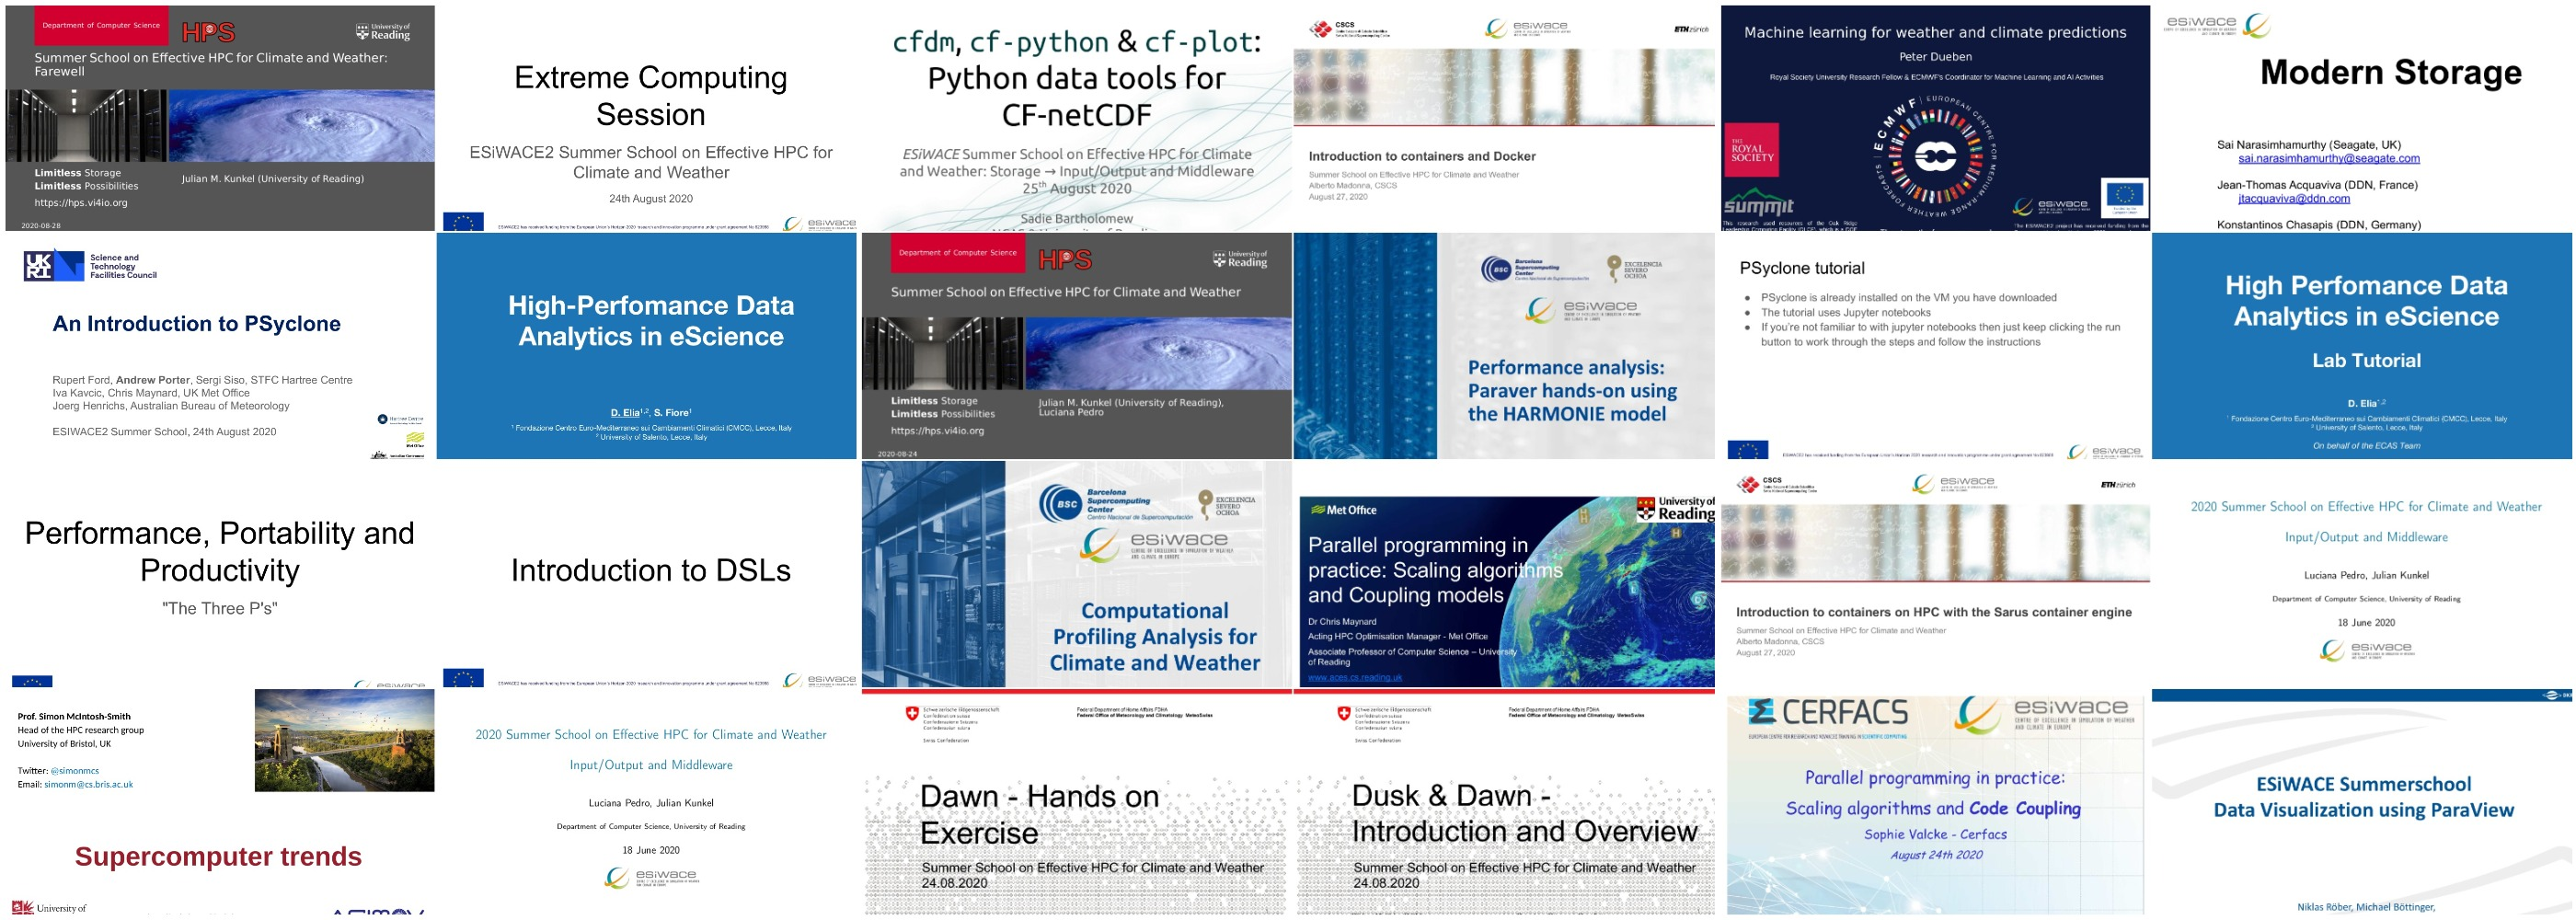
\includegraphics[scale=0.15]{mosaic}
\caption{\href{https://www.photojoiner.net/v/BTvmSc6R}{Snapshot} of first-page presentations.}
\end{table}

The format of the summer school was slightly changed to accommodate the current worldly situation. From Monday to Thursday, a topical session, consisting of an academic lecture and hands-on/lab practicals, was delivered. In total, 18 hours of lecture and 10 hours of hands-on. There was also a virtual visit to ECMWF covering tours to the Computer Hall and the Weather Room. The sessions covered the following topics:

\begin{description}

\item[Monday] Extreme-Scale Computation (STFC, MeteoSwiss) and Parallel Programming in Practice (CERFACS, UREAD).

\item[Tuesday] Modern Storage (Seagate, DDN) and Input/Output and Middleware (UREAD).

\item[Wednesday] Machine Learning (ECMWF) and High-Performance Data Analytics and Visualisation (CMCC, DKRZ).

\item[Thursday] Performance Analysis (BSC) and Containers (ETH Zürich, NCAS).

\end{description}

On Friday, a different format was administered. We organised extra sessions in a Q\&A format for each lab that happened during the week, and we finished the program with a Keynote Talk. Daniel Klocke, from DWD (Germany), presented his work with Global Storm and Ocean Eddy Resolving Coupled Climate Simulations and the contributions of projects DIAMOND and DIAMOND2.

All sessions were recorded and the recordings, together with the presentations and material for each session, are available in the main \href{https://hps.vi4io.org/events/2020/esiwace-school}{summer school webpage}. The links are also available throughout this document, in their respective sessions of the summer school, and in Chapter \ref{ch:material}.

After the event, we asked the participants to fulfil a survey. Here are some of the main numbers and comments about what they most liked about the summer school:

\begin{itemize}

\item 38.5\% said the summer school was better than they were expecting and 46.2\% said it was as good as they were expecting;

\item 92.3\% said they had an excellent or good experience;

\item Selected quotes from attendees:

\begin{itemize}

\item ``The combination of learning the theory, getting some hands-on it, and working with the learned things'';
\item ``The interdisciplinary spirit of the presentations and profound knowledge of people invited to talk'';
\item ``High-quality presentations and I can revisit it when I need on youtube''.

\end{itemize}

\end{itemize}

Chapter \ref{ch:ss2021} is about the summer school 2021. To be done.